
\documentclass[a4paper]{article}
\usepackage[a4paper,top=2cm,bottom=2cm,left=2cm,right=2cm,marginparwidth=2cm]{geometry}
\usepackage{lmodern}
\usepackage{listings}
\usepackage{amsmath}
\usepackage{amssymb}
\usepackage{bm}
\usepackage{textpos} % package for the positioning
\usepackage{tcolorbox}
\usepackage{pgf, tikz}
\usepackage{url}
\usetikzlibrary{arrows, automata}

\setlength{\parindent}{0em}
\setlength{\parskip}{0.3em}

\usepackage{textcomp}
\begin{document}

\lstset{language=Python,upquote=true}

\setlength{\leftskip}{20pt}
\title{Lab 8 Exercise - Exploring Latent Spaces}
\author{Jonathon Hare (jsh2@ecs.soton.ac.uk)}

\maketitle

% \begin{abstract}
% \end{abstract}
% \tableofcontents

This is the exercise that you need to work through \textbf{on your own} after completing the eighth lab session. You'll need to write up your results/answers/findings and submit this to ECS handin as a PDF document along with the other lab exercises near the end of the module (1 pdf document per lab). 

We expect that you \textbf{will use no more than one side} of A4 to cover your responses to \emph{this} exercise. This exercise is worth 5\% of your overall module grade.

\section{Exploring the latent space of a VAE}\label{vae}
In the lab you trained a VAE on Fashion MNIST and perhaps plotted some random samples drawn from the decoder. Because the VAE you created had a two-dimensional latent space you can explore the types of image that get generated from different parts of the $\bm z$ space by systematically sampling it. The image below illustrates what this kind of systematic sampling might look like for a VAE trained on MNIST.
\begin{center}
	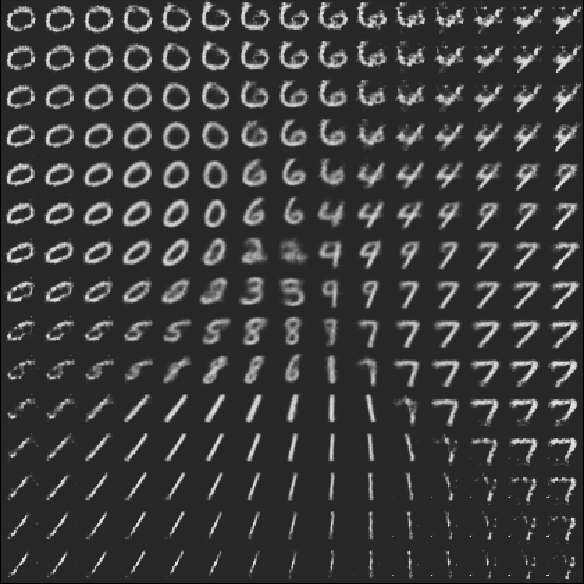
\includegraphics[scale=0.5]{mnist.png}
\end{center}

\begin{tcolorbox}[title=1.1 Systematically sample a VAE (2 marks)]
You're going to create an image like the above, but using the Fashion MNIST VAE you created in the third part of the lab.

With your trained VAE model, use the decoder network to generate images by uniformly sampling the prior from $-4\sigma$ to $+4\sigma$ in both dimensions. Create 21 samples per dimension (so you have a total of 441 2-d $\bm z$ vectors). Draw each reconstruction into a large $588\times588$ image according to the $\bm z$ vector that generated it --- you want the image generated from $\bm z = [-4,4]$ to be in the top left, and the image from $\bm z = [4,-4]$ to be in the bottom right. Save the image you generate and put it into your report.
\end{tcolorbox}

\section{Exploring the code space of a standard auto-encoder}\label{ae}
Autoencoders are not generative models in a true probabilistic sense, but we can still use the decoder part of the network independently by choosing random vectors as input. 

\begin{tcolorbox}[title=2.1 Systematically sample an Autoencoder (2 marks)]
Retrain the autoencoder from part 1 of the lab so that the latent space is 2-d (rather than 64-d). Now uniformly sample the space and create an image just like you did in task 1.1; you should use the same number of samples per dimension (21) and a range of -4 to 4 on each dimension\footnote{there is no particular reason to choose this range; the autoencoder is free to use any real-valued ordinates in its code space, unlike a VAE which has a strong prior drawing latent vectors to the origin.}. Include the picture you generate in the report.
\end{tcolorbox}

\begin{tcolorbox}[title=2.2 Compare the latent spaces of the VAE and autoencoder (1 mark)]
Look at the two images you generated. Comment on the biggest differences in them and relate this to how the respective models work.
\end{tcolorbox}

\end{document}
